\documentclass[../main.tex]{subfiles}

Iniciando este capítulo, se explica la metodología empleada a lo largo del estudio, pero seguida con más énfasis en la comparativa y resultados, es por ello por lo que se presenta durante este capítulo y no con anterioridad. \\
A continuación, se introducen propiedades relevantes de los IPS para poder evaluar en una comparativa posterior los diferentes sistemas y soluciones. Para un IPS no es suficiente hablar solo de la precisión del sistema, sino que otras características como la exactitud, la cobertura, la complejidad, el coste, etc., son también de gran relevancia. \\
Además, se presentan los retos que debe afrontar un IPS para cumplir con su propósito. \\
Posteriormente, se presentará la comparativa en sí de las diferentes soluciones encontradas, acompañada por el modelo seguido para realizar la misma. La taxonomía valora las diferentes tecnologías según sus propiedades y establece las mejores soluciones según el modelo aplicado. Tanto el modelo como el rango de valores de las propiedades variará entre diferentes aplicaciones. En este capítulo, se presentan de forma genérica la comparativa, será en el próximo capitulo cuando se concretará una aplicación y se aplicará la comparativa explicada para la misma.

\section{Metodología} \label{section:metodologia}
La metodología aplicada en el estudio para el análisis de soluciones se conoce como \emph{trade-offs}. Es un procedimiento típico en ingeniería a la hora de comparar soluciones que trata de analizar las fortalezas y debilidades de las alternativas para encontrar una solución de compromiso. \\
En este estudio, la metodología seguida consiste en los siguientes pasos: 

\begin{itemize}
    \item Entender el contexto.
    \item Definir opciones existentes.
    \item Definir el criterio.
    \item Fijar pesos del criterio.
    \item Extraer puntuación y resultados.
    \item Análisis de resultados y toma de decisiones.
\end{itemize}

La figura \ref{fig:metodologia} presenta de forma esquemática la secuencia con las diferentes fases seguidas en la metodología.

\begin{figure}[H]
    \centering
    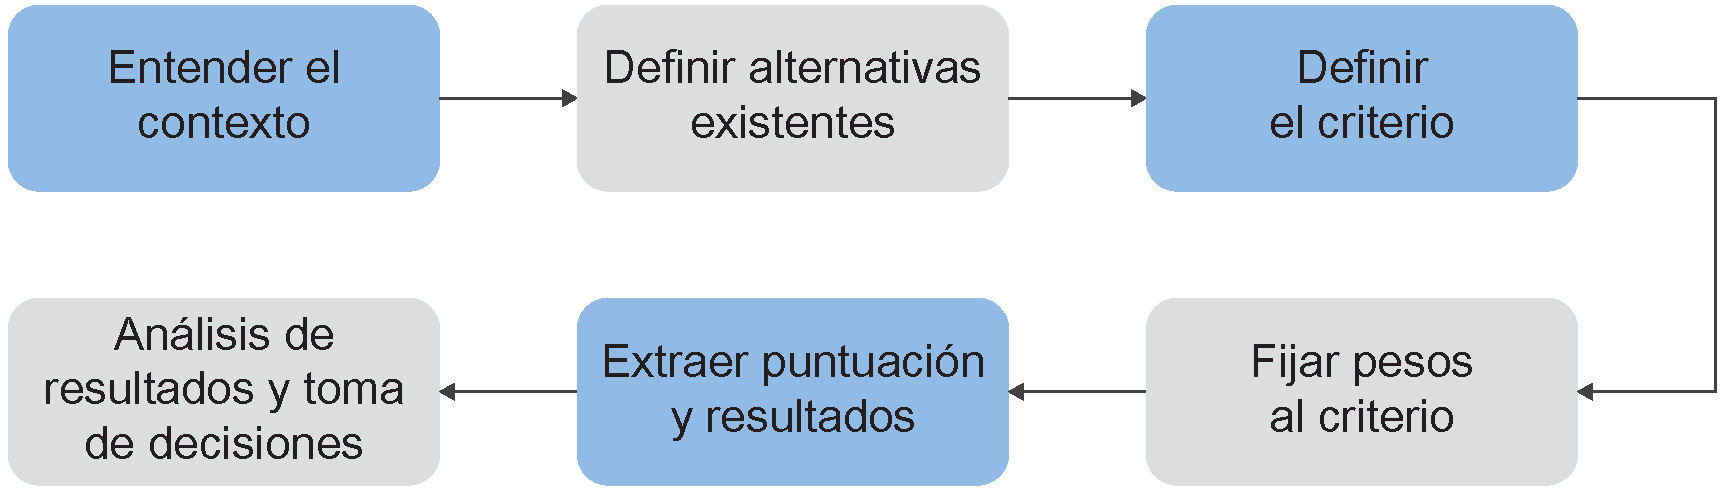
\includegraphics[width=0.8\textwidth]{proceso.pdf}
    \caption{Secuencia de fases de la metodología.}
    \label{fig:metodologia}
\end{figure}

A continuación, se aportará una breve explicación de cada uno de los pasos y se enmarcarán estos en el trabajo.

\subsection*{Entender el contexto}
En primer lugar, es necesario entender la definición del problema y el marco en el que se encuadra el mismo. Comprender los motivos, las causas, los objetivos o los requisitos es imprescindible para llevar a cabo los siguientes pasos. También es esencial identificar todos los factores (internos o externos) que puedan afectar a la toma de decisiones. \\
Discernir las opciones existentes suele considerarse como parte necesaria del contexto, y para su desarrollo es común realizar una lluvia de ideas o \emph{brainstorming}. \\
Durante este estudio, el contexto se ha definido y explicado a lo largo de los Capítulos \ref{chapter:introduccion}, \ref{chapter:tecnicas} e incluso una sección de este capítulo (\ref{section:propiedades})..

\subsection*{Definir opciones existentes}
Tras analizar y entender el contexto, el siguiente paso es definir las diferentes opciones existentes. Estas alternativas pueden haber surgido mediante una lluvia de ideas, un estudio del mercado u otro origen. \\
Las alternativas existentes se han desarrollado a los largo de los Capítulos \ref{chapter:tecnicas} y \ref{chapter:tecnologias}.

\subsection*{Definir el criterio}
En este punto, tanto el contexto como las opciones existentes ya están dominadas. Es el momento de definir el método de elección entre las alternativas, es decir, la forma de evaluar las opciones existentes. El modelo tiene que responder a las preguntas ``¿cuáles son las cualidades más relevantes?'' o ``¿que restricciones existen?''. \\
Existen diversos métodos a seguir para definir el criterio, el seguido en este estudio (durante la Sección \ref{section:mod_baremo}) es uno muy básico. El modelo presentado se reduce en enumerar y agrupar una serie de valores derivados de las propiedades, previamente explicadas en el contexto, acompañadas por su correspondiente coeficiente o peso.

\subsection*{Fijar pesos del criterio}
Probablemente, el paso más importante y delicado dentro de la metodología. El propósito a la hora de fijar los pesos es elegir aquellos que mejor representen las necesidades descritas para obtener los resultados deseados. Sin embargo, esto no es tarea sencilla pues la selección de los pesos puede variar drásticamente en los resultados obtenidos. \\
En este trabajo, los pesos se fijan durante el Capítulo \ref{chapter:estudio}. Con el objetivo de aumentar la robustez de la solución, los pesos considerados inicialmente son modificados y los resultados alterados son comparados entre sí.

\subsection*{Extraer puntuación y resultados}
Tras agregar los pesos para cada criterio, se debe asociar una puntuación a cada valor del criterio para cada opción. Este proceso puede conllevar varias iteraciones pues la puntuación de un valor puede variar al considerar otro posterior. \\
Una vez se hayan valorado todas las opciones, se puede extraer una clasificación con los mejores resultados. En esta memoria, las valoraciones y los resultados se realizan durante el Capítulo \ref{chapter:estudio}.

\subsection*{Análisis de resultados y toma de decisiones}
Finalmente, sobre la clasificación de soluciones obtenidas es necesario un análisis. Habitualmente, la solución con mayor puntuación suele ser la seleccionada, pero no siempre. En ingeniería puede darse el caso que una combinación de soluciones pueda solucionar también el problema. En este caso, la toma de decisiones no es directa. Una posibilidad es repetir la metodología con la combinación de opciones con mayor puntuación. \\
De una forma u otra, es necesario tomar una decisión y seleccionar una solución que resuelva el problema que esté respaldada por la metodología desarrollada. Al igual que sucedía con los dos pasos anteriores, esta fase final se realiza durante el Capítulo \ref{chapter:estudio}.

\section{Propiedades} \label{section:propiedades}

\subsection*{Precisión y exactitud} \label{subsection:precision}
La exactitud es el requisito más importante de los sistemas de posicionamiento. Se refiere a la distancia euclidiana promedio entre la ubicación estimada y la ubicación verdadera, es decir a cuán cerca del valor real se encuentra el valor medido (ver Fig. \ref{fig:accuracy}).
Por lo general, la exactitud se adopta como la métrica de rendimiento, cuanto mayor sea la exactitud, mejor será el sistema. Sin embargo, a menudo existe una compensación entre la exactitud y otras características, ya que se necesita cierto compromiso entre la exactitud adecuada y las otras características.

La precisión se refiere a la dispersión del conjunto de valores obtenidos de mediciones repetidas de una magnitud. Cuanto menor es la dispersión mayor la precisión (Fig. \ref{fig:accuracy}). Es una medida de la robustez del sistema de posicionamiento, ya que revela la variación en su rendimiento durante muchas pruebas. Una medida común de la variabilidad es la desviación estándar de las mediciones y la precisión se puede estimar como una función de ella.

\begin{figure}[h]
    \centering
    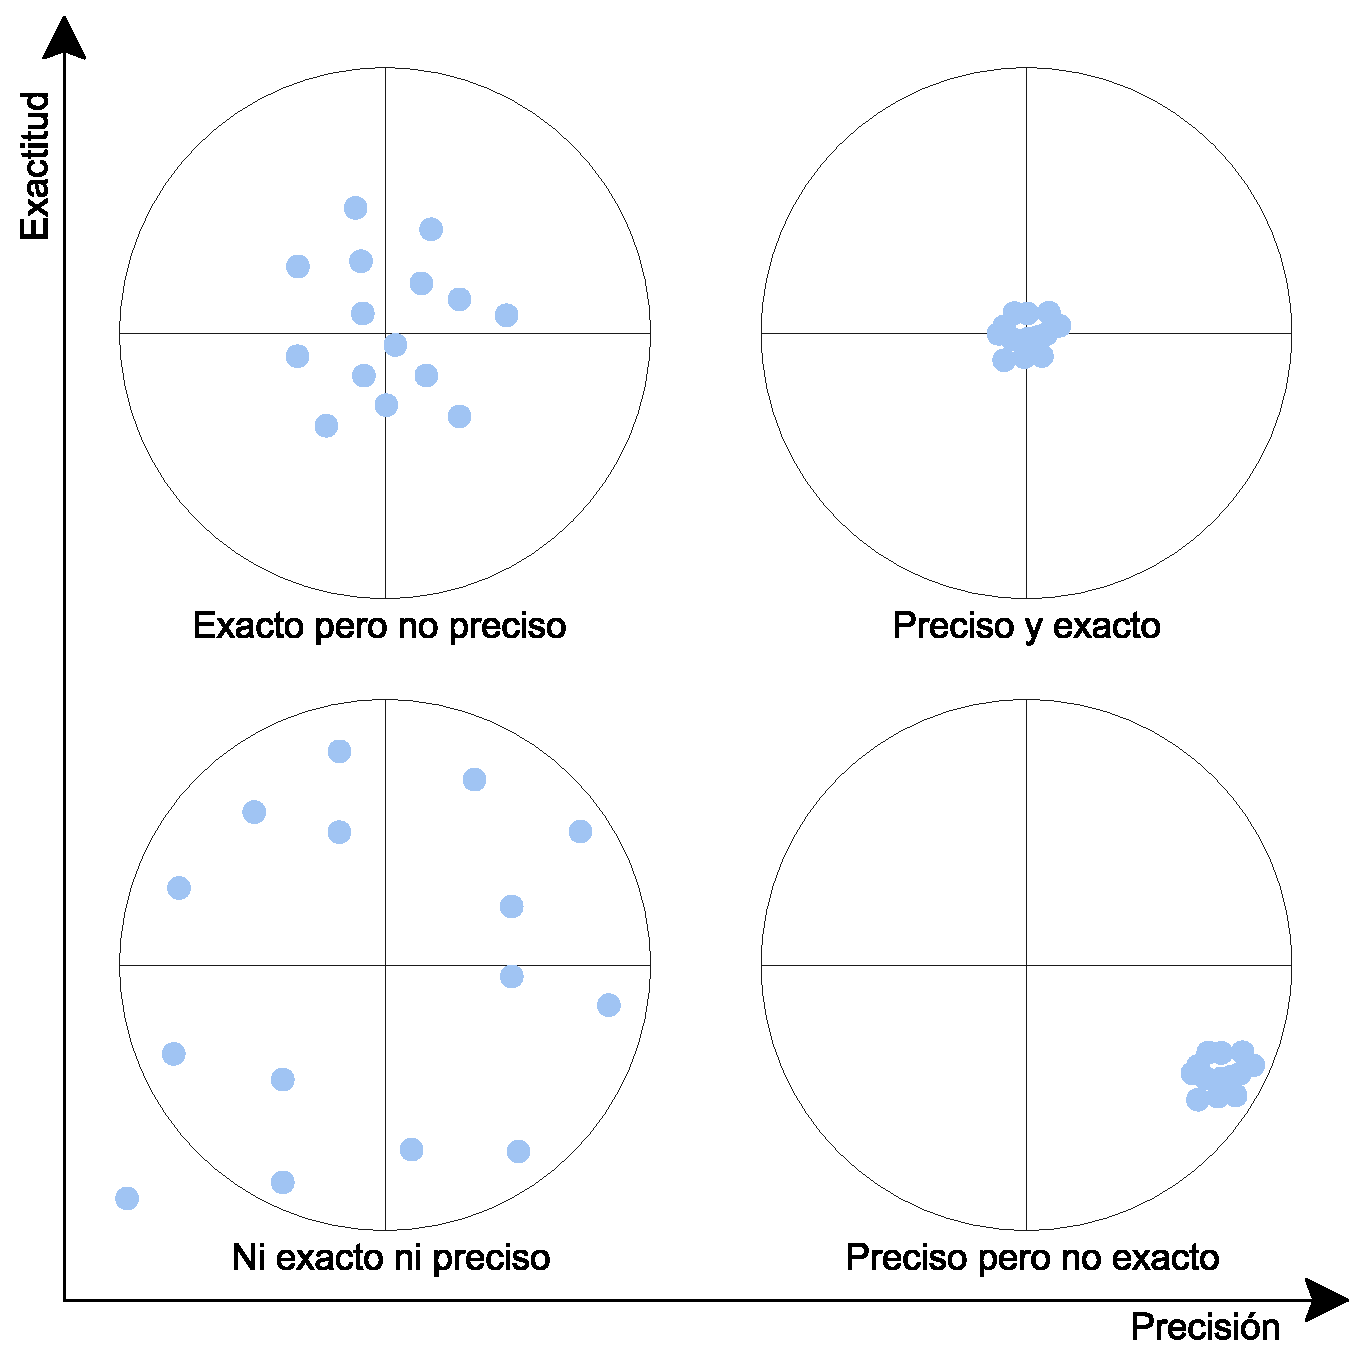
\includegraphics[width=0.6\textwidth]{accuracy.pdf}
    \caption{Precisión frente a exactitud.}
    \label{fig:accuracy}
\end{figure}

\subsection*{Cobertura} \label{subsection:cobertura}
La cobertura, el rango o la escala se refieren a la extensión o área en la cual el sistema puede ubicar un usuario u objeto. Aunque algunas tecnologías pueden ofrecer una amplia cobertura en un entorno ideal, cuando se usan en interiores, su cobertura puede estar limitada por factores ambientales.
Ciertos autores como \emph{Mautz} \cite{Mautz.2012} distinguen la cobertura en las siguientes categorías:

\begin{itemize}
    \item Local: cobertura para una pequeña extensión bien definida, como una habitación o un estadio.
    \item Global: cobertura mundial o internacional para una zona específica. Son los sistemas GNSS los que ofrecen tal cobertura, y como ya se ha mencionado previamente tienen una mal funcionamiento en interiores.
    \item Escalable: sistemas que ofrecen una cobertura incrementable mediante la adición de hardware al sistema. Es importante aclarar que la escalabilidad del sistema no puede afectar a la exactitud del posicionamiento.
\end{itemize}

De esta forma, se han integrado dos características muy cercanas y de gran relevancia para un sistema IPS.

\subsection*{Coste} \label{subsection:coste}
El coste de un sistema de posicionamiento depende de muchos factores. Se considera el coste como la cantidad de recursos invertidos para la instalación y operación de un IPS. Estos recursos pueden ser de diversa naturaleza e incluyen dinero, tiempo, espacio, peso, energía, memoria, etc. \\
Autores como \emph{Brena et al.} \cite{Brena.2017} distinguen dos tipos de coste. En primer lugar, un coste de instalación y mantenimiento, el cual, suele ser un coste incremental y a tener en cuenta con la escalabilidad del sistema. Cabe destacar la existencia de sistemas que carecen de una infraestructura propia y que hacen uso de infraestructuras existentes como la iluminación, el sonido ambiental o redes de puntos de acceso Wi-Fi. \\
En segundo lugar, un coste para el usuario final. En este tipo cabe destacar los sistemas pasivos para el usuario. El término ``pasivo'' puede ser confuso, ya que existen diversos enfoques que hacen uso de tal expresión. Esta pasividad para el usuario final se puede trasladar al peso y consumo, si el sistema no está a bordo del usuario final, a memoria y procesamiento, si el posicionamiento se obtiene en la infraestructura, entre otros.

\subsection*{Complejidad} \label{subsection:complejidad}
La complejidad de un sistema puede atribuirse al hardware, software o procesos computacionales. El coste está muy relacionado con la complejidad, ya que la mayoría de los sistemas de posicionamiento y navegación existentes son complejos en su diseño e implementación, lo que a su vez resulta en un sistema costoso. \\
En concreto, esta comparativa se centra en la complejidad de los procesos computacionales, es decir, la complejidad informática del algoritmo de posicionamiento. Es importante destacar que el cálculo del posicionamiento y el procesamiento del algoritmo puede realizarse en local (unidad móvil) o en remoto (servidor central). Esto conlleva diferentes complejidades asociadas, pues la mayoría de las unidades móviles carecen de gran potencia de procesamiento y de gran batería.

\subsection*{Carga de pago} \label{subsection:payload}
En aplicaciones donde la unidad móvil es un robot autónomo, como los vehículos autónomos no tripulados los cuales son el objeto a posicionar en este trabajo, la carga de pago puede ser crucial para el sistema. En concreto, el tipo de carga de pago puede ser muy diverso, con tamaños, pesos y consumos muy diferentes. \\
En este estudio, se considera ventajosa aquella carga de pago que interfiera o modifique al mínimo a la unidad móvil. Una carga de pago ideal sería aquella inexistente, pues no alteraría la configuración de la unidad móvil.

\subsection*{Otros} \label{subsection:otros}
Existen otros muchos parámetros para comparar los IPS, y dado que es imposible explicarlos todos, se mencionan a continuación los más utilizados en artículos de referencia en este campo. Bien es cierto que varias propiedades ya han sido introducidas en los parámetros desarrollados. De esta forma, destacamos: privacidad, robustez, usabilidad, escalabilidad, identificación, latencia, tasa de refresco, necesidad de infraestructura, cálculo de posicionamiento en local, interferencias o limitaciones. 


\section{Retos} \label{section:retos}
La rama de la ingeniería que se encarga del diseño de sistemas para controlar el movimiento de vehículos es el GNC (Guiado, Navegación y Control). Este trabajo abarca la función de navegación. \\
La definición de navegación es tan diversa como su actividad. Muchos autores han definido este término a lo largo de la historia. Bien es cierto que existen puntos comunes en estas definiciones. De ellos se puede extraer, la navegación aérea es el proceso de dirigir una aeronave en vuelo desde una posición inicial hasta una posición final, siguiendo una ruta determinada y cumpliendo además con ciertos requisitos de seguridad y eficiencia. Es sencillo inferir de la definición anterior los tres elementos principales en la navegación, posición inicial, posición de destino y la ruta a seguir, o la información necesaria para determinar la ruta. Estos tres elementos, no son más que el vector de estado propio. \\
Para determinar el vector de estado es necesario conocer la posición, la orientación y la velocidad, entre otros. En este punto entra en escena los IPS, pues son estos sistemas los que deben determinar la posición y la orientación. \\
Por último, en entornos en interiores es importante la detección de obstáculos, ya que la densidad de obstáculos es mucho mayor debido a la masa de objetos estáticos. Además, el entorno puede ser dinámico, cambiante. Por ejemplo, abrir una ventana podría afectar el ambiente al cambiar la ubicación de los obstáculos, la intensidad de la iluminación y la distribución de la presión.\\
A modo de resumen, los retos a los que tiene que hacer frente un IPS son la determinación de la \emph{posición}, la determinación de la \emph{orientación} y la detección de \emph{obstáculos}.

\subsection*{Posicionamiento} \label{subsection:posicion}
Entendemos por posicionamiento como la determinación de la posición de un objeto o una persona. Siendo la \emph{posición} como la localización de un objeto en el espacio o en el espacio y en el tiempo. \\
Autores como \emph{Hightower et al.} \cite{Hightower.2001} o \emph{Mautz} \cite{Mautz.2012} distinguen dos tipos de posicionamiento. Por un lado, diferencian en función de la información aportada por el sistema entre posicionamiento simbólico y físico. El posicionamiento físico aporta algún tipo de magnitud para posicionar el objeto, mientras que el posicionamiento simbólico aporta ideas abstractas de donde se encuentra algo, por ejemplo, en el laboratorio, en frente del aulario, etc. Por otro lado, en relación del sistema de referencia usado se distingue entre posicionamiento absoluto y relativo. En el posicionamiento absoluto se utiliza un único sistema de referencia global para todos los objetos, mientras que en el posicionamiento relativo cada objeto tiene su propio marco de referencia local. \\
Para representar la posición (\emph{física}) es común utilizar una magnitud vectorial mediante el vector de posición. Este vector puede tener dos, tres o cuatro variables en función de lo que queramos representar; el plano ($x, y$), el espacio ($x, y, z$) y el espacio-tiempo ($x, y, z, t$) respectivamente. \\
La calidad del posicionamiento suele expresarse en la resolución de metros $m$ medida mediante las propiedades de precisión y exactitud ya mencionadas.

\subsection*{Orientación} \label{subsection:orientacion}
La orientación o actitud es la diferencia angular medida entre el eje de un objeto móvil y la línea de horizonte de la Tierra, la dirección de movimiento, otros objetos, etc.
En la aeronavegación, debido a que el objeto es capaz de rotar alrededor de tres ejes perpendiculares entre si, se distinguen tres medidas. Estas rotaciones son cabeceo, guiñada y alabeo. \\
La calidad de la orientación suele expresarse en la resolución de grados (\textordmasculine) medida mediante las propiedades de precisión y exactitud ya mencionadas.

\subsection*{Obstáculos} \label{subsection:obstaculos}
Por último, la detección y evasión de obstáculo es desafío más complejo al que se enfrenta un IPS. Son múltiples y muy diversas la naturaleza de los obstáculos con los que un objeto móvil se puede encontrar, desde paredes hasta otros objetos móviles. Como ya se ha adelantado, los entornos en interiores poseen una densidad de obstáculos mayor que en exteriores, a la par de que el entorno es dinámico y puede sufrir modificaciones.
El problema de evasión de colisiones puede ser unidimensional, bidimensional o tridimensional, aumentando la complejidad del mismo. \\

\section{Taxonomía de las tecnologías de los IPS} \label{section:clasificacion}
Una vez introducidos los criterios de evaluación de los sistemas, se presenta una tabla  comparativa (Tab. \ref{table:taxonomy}) con las diferentes tecnologías tratadas durante el Capítulo \ref{chapter:tecnologias}. Los valores mostrados en la tabla se justifican en las diferentes citas añadidas. \\

Cabe destacar que se ha hecho una distinción previa en alguna tecnología presentada en la Tabla \ref{table:taxonomy}, las cuales se explicarán a continuación. \\
En primer lugar, debido a la gran variedad de sistemas con diferentes características dentro del \emph{motion tracking}, se ha divido en dos categorías (\emph{optical marked motion tracking} y \emph{optical motion tracking}), de mayor exactitud con alto coste asociado y otra de coste y exactitud reducido. Por un lado, los sistemas con mayores prestaciones suelen utilizar tecnologías híbridas y con marcadores reflectantes, de ahí el nombre que se le ha otorgado en este trabajo. Por otro lado, dentro de las tecnologías con menores prestaciones el abanico de opciones sigue siendo enorme debido a la gran variedad de cámaras disponibles. Para este trabajo, se ha seleccionado una que cumple con los requisitos de exactitud con un coste asociado moderado. \\
En segundo lugar, se ha distinguido entre la navegación basada en marcadores en función de su configuración, activa o pasiva. Las diferencias son claras, mientras la configuración activa lleva un dispositivo óptico a bordo y los marcadores se encuentran en el entorno, en la configuración pasiva sucede al contrario. Las principales diferencias entre ambos son la carga de pago y el rango, como se puede observar en la tabla. \\
En tercer lugar, se ha hecho distinción entre los sistemas de identificación por radio-frecuencia en función de su configuración, activa o pasiva. Al igual que sucedía con el caso anterior, la configuración activa lleva el lector RFID a bordo y las etiquetas se encuentran en el entorno, mientras que en la configuración pasiva sucede a la inversa, los lectores se encuentran en el entorno. Las principales diferencias vuelven a ser la carga de pago y el rango asociado a cada configuración. \\
Además, en la Tabla \ref{table:taxonomy} no se han incluido dos tecnologías tratadas en las Sección \ref{section:rf}, NFC y WSN. Ambas tecnologías se han considerado prescindibles debido a su similitud con RFID y WLAN, respectivamente, y sus menores prestaciones con respecto a estas. \\

\small{
\begin{landscape}
    
    \begin{ThreePartTable}
    \renewcommand\TPTminimum{\textwidth}
    %% Arrange for "longtable" to take up full width of text block
    \setlength\LTleft{0pt}
    \setlength\LTright{0pt}
    \setlength\tabcolsep{0pt}

    \begin{TableNotes}
      \item[a] Sensible a errores. Los errores se acumularán e irán en aumento.
    \end{TableNotes}
    
    \begin{longtable}{ l @{\extracolsep{\fill}} *{8}{c} }
    
    \caption{Clasificación de las tecnologías en los IPS.}
    \label{table:taxonomy}\\
    \toprule
                               & \thead{Carga}   & \multicolumn{2}{c}{\thead{Coste}} &               &                     & \thead{Posicionamiento} & \thead{Actitud} & \thead{Obstáculos} \\
            \thead{Tecnología} & \thead{de pago} & \thead{IM}           & \thead{UF} & \thead{Rango} & \thead{Complejidad} & \thead{(Exactitud)}     & \thead{(Si/no)} & \thead{(Si/No)}    \\
    \midrule
    \endfirsthead
    
    \multicolumn{6}{c}{{\textit{\tablename\ \thetable{} -- continuación de la hoja anterior} }}\\
    \toprule
                               & \thead{Carga}   & \multicolumn{2}{c}{\thead{Coste}} &               &                     & \thead{Posicionamiento} & \thead{Actitud} & \thead{Obstáculos} \\
            \thead{Tecnología} & \thead{de pago} & \thead{IM}           & \thead{UF} & \thead{Rango} & \thead{Complejidad} & \thead{(Exactitud)}     & \thead{(Si/no)} & \thead{(Si/No)}    \\
    \midrule
    \endhead

    \midrule[\heavyrulewidth]
    \multicolumn{8}{r}{\textit{---continua en la siguiente hoja}}\\
    \endfoot  

    \midrule[\heavyrulewidth]
    \insertTableNotes
    \endlastfoot

        \multirow{2}{*}{Infrarrojos}  & Medio              & \multirow{2}{*}{-}    & Medio                 & \multirow{2}{*}{Local}     & \multirow{2}{*}{-} & 1D, Media (10cm) & \multirow{2}{*}{No} & \multirow{2}{*}{No} \\
                                      & (5-10g)            &                       & (20\EURcr)            &                            &                    & \cite{gorostiza.2011} &    & \\ \\
            
        \multirow{2}{*}{Luz visible}  & Ligero             & \multirow{2}{*}{Alto} & Bajo                  & \multirow{2}{*}{Local}     & Alto               & 3D, Media (20cm) & \multirow{2}{*}{No}   & \multirow{2}{*}{No} \\
                                      & (0,39g)            &                       & (\<5\EURcr)           &                            & computo            & \cite{liu.2010vlc, zhang.2014} & & \\ \\
            
        \multirow{2}{*}{\emph{Optical flow}} & Pesado      & \multirow{2}{*}{-}    & Alto                  & \multirow{2}{*}{Escalable} & \multirow{2}{*}{-} & 2D, Alta (1mm) & \multirow{2}{*}{Si} & \multirow{2}{*}{No} \\
                                      & (17g)              &                       & (100\EURcr)           &                            &                    & \cite{li.2018novel, mcguire.2017} &  & \\ \\
            
        \emph{Optical motion}         & \multirow{2}{*}{-} & Medio                 & \multirow{2}{*}{-}    & \multirow{2}{*}{Local}     & \multirow{2}{*}{-} & 3D, Alta (cm) & \multirow{2}{*}{No} & \multirow{2}{*}{No} \\
        \emph{tracking}               &                    & (20\EURcr/cam)        &                       &                            &                    & \cite{mustafah.2012, tisse.2005} & & \\ \\
            
        \emph{Optical marked}         & \multirow{2}{*}{-} & Alto                  & \multirow{2}{*}{Bajo} & \multirow{2}{*}{Local}     & \multirow{2}{*}{-} & 3D, Alta (20 $\mu$m) & \multirow{2}{*}{Si} & \multirow{2}{*}{Si} \\
        \emph{motion tracking}        &                    & (3000\EURcr/cam)      &                       &                            &                    & \cite{vicon, optitrack} & & \\ \\
            
        \emph{Marked-based}           & Medio              & \multirow{2}{*}{Bajo} & Alto                  & \multirow{2}{*}{Escalable} & \multirow{2}{*}{-} & 3D, Alta (cm) & \multirow{2}{*}{Si}  & \multirow{2}{*}{No} \\
        (Activo)                      & (10g)              &                       & (80\EURcr)            &                            &                    & \cite{Mautz.2012} &                  & \\ \\
        
        \emph{Marked-based}           & \multirow{2}{*}{-} & Alto                  & \multirow{2}{*}{Bajo} & \multirow{2}{*}{Local}     & \multirow{2}{*}{-} & 3D, Alta (cm) & \multirow{2}{*}{Si}  & \multirow{2}{*}{No} \\
        (Pasivo)                      &                    & (80\EURcr/cam)        &                       &                            &                    & \cite{Mautz.2012} &                  & \\ \\
        
        \multirow{2}{*}{\emph{Vision-based}} & Pesado      & \multirow{2}{*}{-}    & Medio                 & \multirow{2}{*}{Escalable} & Alto               & 3D, Alta (cm) & \multirow{2}{*}{Si} & \multirow{2}{*}{Si} \\
                                      & (15g)              &                       & (20\EURcr)            &                            & computo            & \cite{Mautz.2012, mcguire.2017} & & \\ \\
        
        \multirow{2}{*}{LiDAR}        & Inviable           & \multirow{2}{*}{-}    & Muy Alto              & \multirow{2}{*}{Escalable} & Alto               & 3D, Alta (1mm) & \multirow{2}{*}{No} & \multirow{2}{*}{Si} \\
                                      & (830g)             &                       & (5000\EURcr)          &                            & computo            & \cite{schmitt.2010igps} &            & \\
        
        \multirow{2}{*}{Ultrasonidos} & Medio              & \multirow{2}{*}{Bajo} & Medio                 & \multirow{2}{*}{Escalable} & \multirow{2}{*}{-} & 3D, Alta (1cm) & \multirow{2}{*}{No} & \multirow{2}{*}{No} \\
                                      & (5g)               &                       & (30\EURcr)            &                            &                   & \cite{priyantha.2000, fukuju.2003, minami.2004} & & \\ \\
        
        \multirow{2}{*}{Audible}      & Medio              & \multirow{2}{*}{Bajo} & Medio                 & \multirow{2}{*}{Local}     & \multirow{2}{*}{-} & 3D, Media (50cm) & \multirow{2}{*}{No}  & \multirow{2}{*}{No} \\
                                      & (5g)               &                       & (30\EURcr)            &                            &                    & \cite{mandal.2005,peng.2012, liu.2013guoguo} & & \\ \\
        
        \multirow{2}{*}{Magnética}    & \multirow{2}{*}{-} & Alto                  & \multirow{2}{*}{-}    & \multirow{2}{*}{Local}     & \multirow{2}{*}{-} & 3D, Baja (2m) & \multirow{2}{*}{No} & \multirow{2}{*}{No} \\
                                      &                    & (300\EURcr)           &                       &                            &                    & \cite{indooratlas} & & \\ \\

        \multirow{2}{*}{WLAN}         & Medio              & \multirow{2}{*}{Bajo} & Alto                  & \multirow{2}{*}{Escalable} & \multirow{2}{*}{-} & 3D, Baja (1-5m) & \multirow{2}{*}{No} & \multirow{2}{*}{No} \\
                                      & (10g)                 &                       & (100\EURcr)           &                            &                    & \cite{bahl.2000} &         & \\ \\
        
        \multirow{2}{*}{Bluetooth}   & Medio              & Medio                  & Medio                 & \multirow{2}{*}{Escalable} & \multirow{2}{*}{-} & 3D, Baja (1-5m) & \multirow{2}{*}{No} & \multirow{2}{*}{No} \\
                                     & (13g)              & (20\EURcr/ant)         & (20\EURcr)            &                            &                    & \cite{ibeacon} &           & \\ \\
        
        \multirow{2}{*}{RFID activo} & Pesado             & Bajo                   & Alto                  & \multirow{2}{*}{Escalable} & \multirow{2}{*}{-} & 3D, Baja (1-2m) & \multirow{2}{*}{No} & \multirow{2}{*}{No} \\
                                     & (22g)              & (2\EURcr/etiqueta)     & (200\EURcr)           &                            &                    & \cite{Hightower.2001, ni.2003landmarc} & & \\ \\
            
        \multirow{2}{*}{RFID pasivo} & Ligero             & Alto                   & Bajo                  & \multirow{2}{*}{Local}     & \multirow{2}{*}{-} & 3D, Baja (1-2m) & \multirow{2}{*}{No} & \multirow{2}{*}{No} \\
                                     & (5g)                 & (200\EURcr/lector)     & (2\EURcr)             &                            &                    & \cite{Hightower.2001, ni.2003landmarc} & & \\ \\
        
        \multirow{2}{*}{UWB}         & Ligero             & Medio                  & Medio                 & \multirow{2}{*}{Escalable} & \multirow{2}{*}{-} & 3D, Media (10cm) & \multirow{2}{*}{No} & \multirow{2}{*}{No} \\
                                     & (1,4g)             & (30-100\EURcr/ant)     & (30-100\EURcr)        &                            &                    & \cite{ruiz.2017, decawave} & & \\ \\
        
        \multirow{2}{*}{IMU}         & Medio              & \multirow{2}{*}{-}     & Medio                 & \multirow{2}{*}{Escalable} & \multirow{2}{*}{-} & \multirow{2}{*}{3D, Alta\tnote{a}} & \multirow{2}{*}{Si}  & \multirow{2}{*}{No} \\
                                     & (10g)              &                        & (20\EURcr)            &                            &                    &                    &                      & \\
    \end{longtable}
    \end{ThreePartTable}
\end{landscape}
}
\normalsize

Con el objetivo de aclarar los posibles valores con los que se han clasificado las diferentes tecnologías, se presenta una segunda tabla (Tab. \ref{table:explanation}) que recoge los niveles existentes para cada atributo examinado.

\begin{table}[h]
    \centering
    \begin{threeparttable}
        \begin{tabular}{l c c}
            \toprule
            \thead{Propiedad} & \thead{Valores} & \thead{Rango de valores}\\
            
            \midrule
            \multirow{5}{*}{Carga de pago} & Inviable   & $>$50g \\
                                           & Pesado     & 15-50g \\
                                           & Medio      & 5-15g  \\
                                           & Ligero     & 0-5g   \\
                                           & Nulo       & 0g     \\
            \cline{1-3}
            \multirow{4}{*}{Coste} & Alto  & $>$50\EUR \\
                                   & Medio & 10-50\EUR \\
                                   & Bajo  & 0-10\EUR  \\
                                   & Nulo  & 0\EUR     \\
                                   
            \cline{1-3}
            \multirow{3}{*}{Rango} & Local     & \multirow{3}{*}{Ver sección \ref{subsection:cobertura}} \\
                                   & Escalable & \\
                                   & Global    & \\
            \cline{1-3}
            \multirow{3}{*}{Complejidad} & Software & \multirow{3}{*}{Ver sección \ref{subsection:complejidad}} \\ 
                                         & Hardware & \\ 
                                         & Computo  & \\
            \cline{1-3}
            \multirow{3}{*}{Exactitud} & Baja  & Metros o superior      \\
                                       & Media & De decímetros a metros \\
                                       & Alta  & Centímetros o inferior \\
            \cline{1-3}
            \multirow{2}{*}{Actitud} & No & Detección de la orientación  \\
                                     & Si & de la aeronave \\
            \cline{1-3}
            \multirow{2}{*}{Obstáculos} & No & Detección y evasión \\
                                        & Si & de obstáculos \\
            \bottomrule
            \addlinespace[1ex]
        \end{tabular}
        
    \end{threeparttable}
    
    \caption{Valores y su correspondiente rango para las propiedades de las tecnologías.}
    \label{table:explanation}
    \end{table}

Es importante mencionar que, de forma intencionada, se han obviado ciertos aspectos sobre las tablas presentadas hasta ahora en la sección. Pues los rango de valores asociados a las propiedades de carga de pago, coste y exactitud pueden variar en función de la aplicación especifica. Por el momento, sin una aplicación específica sobre la que trabajar, se ha presentado unos valores que pueden resultar contradictorios, pero que se justificarán en la siguiente sección cuando se presente la aplicación seleccionada en este trabajo. La decisión de presentar las tablas en esta sección y no en la siguiente radica en el intento de crear una comparativa general sin tener en cuenta la aplicación específica.

\section{Modelo y baremo} \label{section:mod_baremo}
En esta sección, se aportará un modelo y baremación a la Tabla \ref{table:taxonomy} con el objetivo de exponer de forma más sencilla sistema de evaluación a las tecnologías presentadas y poder extraer de estas soluciones las que mejor se adapten al problema particular. Para ello, es necesario definir el modelo y la baremación, que se presentan a continuación. \\
Son el modelo y el baremo lo que variará de una aplicación a otra. En función de la utilidad del sistema, será necesario dar más importancia a ciertas propiedades pues su uso será más limitante.

\subsection*{Modelo} \label{subsection:modelo}
Antes de iniciar el proceso de evaluación, es importante marcar los requisitos a los que el sistema se enfrentará. De esta forma, se ha decidido simplificar el sistema en dos aspectos. En primer lugar, dentro de los tres desafíos que se han presentado en la Sección \ref{section:retos}, se ha decido abordar solamente el posicionamiento y actitud, obviando en primera instancia la detección y evasión de obstáculos.
En segundo lugar, se ha eliminado la complejidad de los requisitos a valorar. El motivo principal de esta decisión es que no se considera un requisito limitante para las tecnologías debido a los avances existentes en computación. \\
El hecho de eliminar tales requisitos es, como ya se ha mencionado, simplemente con el objetivo facilitar un análisis inicial de las tecnologías. En ningún momento se descarta la posibilidad de rescatar estos u otros requisitos para un estudio posterior con más profundidad, o para un segundo análisis de las mejores tecnologías obtenidas de esta primera comparación. \\

Tras presentar los objetivos a los que se hará frente en este estudio, se puede dar paso al modelo de evaluación o puntuación que se aplicará a las diferentes tecnologías ya presentadas. El modelo matemático es el siguiente:

\begin{equation}
    \alpha CP + \beta IM + \gamma UF + \delta RAN + \mu POS + \nu ACT + \omega OBS
    \label{eq:modelo}
\end{equation}

, siendo $CP$ la carga de pago, $IM$ el coste de instalación y mantenimiento, $UF$ el coste para el usuario final, $RAN$ el rango, $POS$ el posicionamiento, $ACT$ la actitud y $OBS$ los obstáculos, todos estos con los valores normalizados sobre uno. Y siendo $\alpha$, $\beta$, $\gamma$, $\delta$, $\mu$, $\nu$ y $\omega$ coeficientes asociados al modelo, con un valor variable en función de los requerimientos específicos de la aplicación.

\subsection*{Baremo} \label{subsection:baremo}
Para presentar de forma más clara el baremo establecido, se ha recuperado la Tabla \ref{table:explanation} sobre la cual se han realizado unas pequeñas modificaciones para obtener la nueva Tabla \ref{table:baremo}.

\begin{table}[h]
    \centering
    \begin{threeparttable}
        \begin{tabular}{l c c}
            \toprule
            \thead{Propiedad} & \thead{Valores} & \thead{Baremo}\\
            
            \midrule
            \multirow{5}{*}{Carga de pago} & Inviable   & 0 \\
                                           & Pesado     & 1 \\
                                           & Medio      & 2 \\
                                           & Ligero     & 3 \\
                                           & Nulo       & 4 \\
            \cline{1-3}
            \multirow{4}{*}{Coste} & Alto  & 0 \\
                                   & Medio & 1 \\
                                   & Bajo  & 2 \\
                                   & Nulo  & 3 \\
            \cline{1-3}
            \multirow{3}{*}{Rango} & Local     & 0 \\
                                   & Escalable & 1 \\
                                   & Global    & 2 \\
            \cline{1-3}
            \multirow{3}{*}{Exactitud} & Baja  & 0 \\
                                       & Media & 1 \\
                                       & Alta  & 2 \\
            \cline{1-3}
            \multirow{2}{*}{Actitud} & No & 0 \\
                                     & Si & 1 \\
            \cline{1-3}
            \multirow{2}{*}{Obstáculos} & No & 0 \\
                                        & Si & 1 \\
            \bottomrule
            \addlinespace[1ex]
        \end{tabular}
        
    \end{threeparttable}
    
    \caption{Baremo para las propiedades de las tecnologías.}
    \label{table:baremo}
\end{table}

Esta tabla no se puede entender sin tener en cuenta el rango de valores de la Tabla \ref{table:explanation} pues una modificación en estos afecta de forma directa al baremo establecido. Así pues, aunque el rango de valores no se muestre en esta tabla por razones de simplificar la misma, forma también parte del baremo. \\
Como es obvio pensar, los valores superiores representan mejores propiedades que los inferiores. Así pues, una carga de pago nula (\emph{4}) es preferible a una carga inviable (\emph{0}). \\

